\documentclass[12pt]{beamer}

%-------------------------------------------------
%   THEMES & PACKAGES
%-------------------------------------------------
\usetheme[progressbar=frametitle]{metropolis}
\usepackage{graphicx}
\usepackage{subcaption}

%-------------------------------------------------
%   TITLE
%-------------------------------------------------
\title{Research and Development}
\subtitle{Possible Approaches}
\date{\today}
\author{Minh Nguyen}
\titlegraphic{\hfill
\includegraphics[height=0.7cm]{../../../images/h-brs-logo.jpg}}

%-------------------------------------------------
%   BEGIN
%-------------------------------------------------
\begin{document}

%-------------------------------------------------
\maketitle

\begin{frame}{Recurrent Neural Networks}
    \begin{alertblock}{}
        \begin{itemize}
            \item Connects the neurons' outputs to their inputs and iteratively train them using ``back-propagation-through-time'' (BPTT)
            \item Is the basic deep learning model from which all the following methods are derived
        \end{itemize}
    \end{alertblock}
\end{frame}

\begin{frame}{Recurrent Neural Networks}
    \begin{alertblock}{Architecture Illustration}
        \begin{figure}[t!]
            \centering
            \setlength{\fboxsep}{1pt}%
            \setlength{\fboxrule}{0.5pt}%
            \fbox{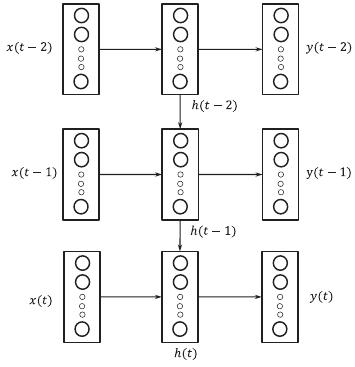
\includegraphics[height=5.0cm]{../../images/laengkvist14-reviewDeepLearning-fig4.png}}
            \caption{Recurrent Neural Network (RNN) \cite{langkvist2014review}}
        \end{figure}
    \end{alertblock}
\end{frame}

\begin{frame}{Long Short-Term Memory}
    \begin{alertblock}{}
        \begin{itemize}
            \item First introduced in \cite{Hochreiter:1997:LSM:1246443.1246450}
            \item Each recurrent unit is a memory cell with:
            \begin{itemize}
                \item an input gate to ``protect against irrelevant inputs'' \cite{Hochreiter:1997:LSM:1246443.1246450}
                \item an output gate to ``protect other hidden units from irrelevant memory'' \cite{Hochreiter:1997:LSM:1246443.1246450}
                \item a forget gate allowing the memory cell to reset as appropriate \cite{Gers:2000:LFC:1121912.1121915}
            \end{itemize}
            \item Successful application in many temporal problems \cite{DBLP:journals/corr/Graves13,conf/icml/JozefowiczZS15}
        \end{itemize}
    \end{alertblock}
\end{frame}

\begin{frame}{Long Short-Term Memory}
    \begin{alertblock}{Architecture Illustration}
        \begin{figure}[t!]
            \centering
            \setlength{\fboxsep}{1pt}%
            \setlength{\fboxrule}{0.5pt}%
            \begin{subfigure}[t]{0.5\textwidth}
                \centering
                \fbox{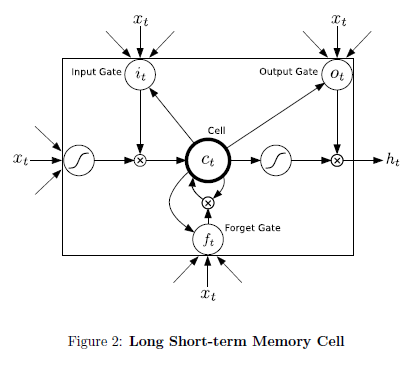
\includegraphics[height=4.5cm]{../../images/Graves13-fig2-lstm_arch.png}}
                \caption{By Graves \cite{DBLP:journals/corr/Graves13}}
            \end{subfigure}%
            \begin{subfigure}[t]{0.5\textwidth}
                \centering
                \fbox{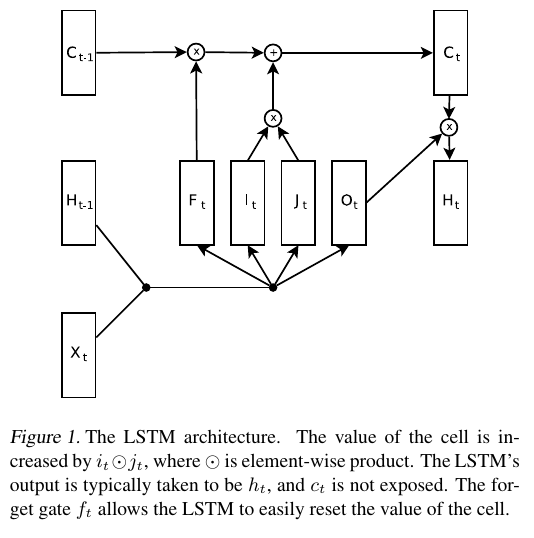
\includegraphics[height=4.5cm]{../../images/jozefowicz15-fig1.png}}
                \caption{By Jozefowicz et al \cite{conf/icml/JozefowiczZS15}}
            \end{subfigure}
            \label{fig:sub1}
            \caption{Long Short-Term Memory (LSTM)}
        \end{figure}
    \end{alertblock}
\end{frame}

\begin{frame}{Gated Recurrent Unit}
    \begin{alertblock}{}
        \begin{itemize}
            \item GRU is proposed by \cite{cho14GRU}, is motivated by LSTM and simpler to compute and implement
            \item Each unit contains:
            \begin{itemize}
                \item a reset gate which forces the unit to forget the previous hidden states when appropriate
                \item an update gate which controls how much information is carried from previous to current hidden state.
               \end{itemize}
        \end{itemize}
    \end{alertblock}
\end{frame}

\begin{frame}{Gated Recurrent Unit}
    \begin{alertblock}{Architecture Illustration}
        \begin{figure}[t!]
            \centering
            \setlength{\fboxsep}{1pt}%
            \setlength{\fboxrule}{0.5pt}%
            \begin{subfigure}[t]{0.5\textwidth}
                \centering
                \fbox{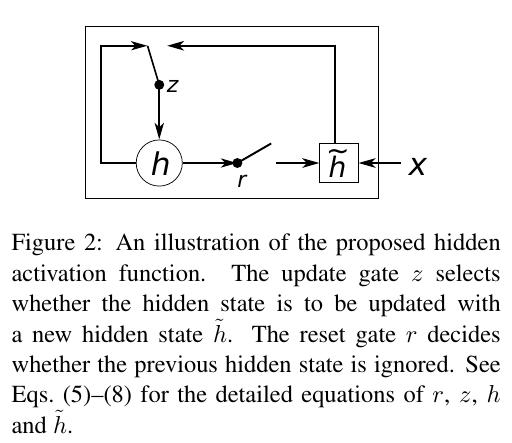
\includegraphics[height=4.5cm]{../../images/cho14-PhraseRepresentGRU-fig2.png}}
                \caption{By Cho \cite{cho14GRU}}
            \end{subfigure}%
            \begin{subfigure}[t]{0.5\textwidth}
                \centering
                \fbox{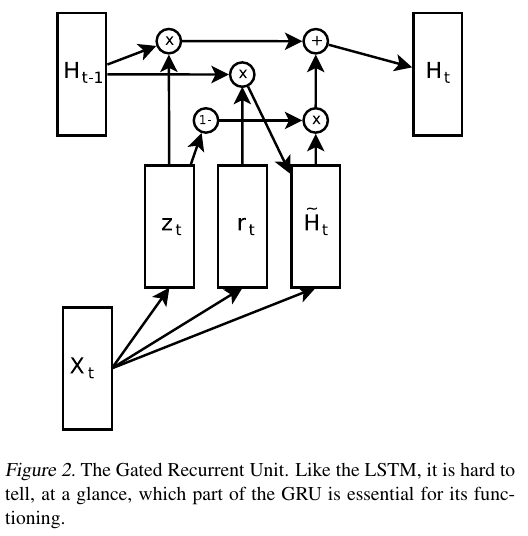
\includegraphics[height=4.5cm]{../../images/jozefowicz15-fig2.png}}
                \caption{By Jozefowicz et al \cite{conf/icml/JozefowiczZS15}}
            \end{subfigure}
            \label{fig:sub1}
            \caption{Long Short-Term Memory (LSTM)}
        \end{figure}
    \end{alertblock}
\end{frame}

\begin{frame}{Hessian-free Optimization}
    \begin{alertblock}{}
        \begin{itemize}
            \item HF for deep learning is introduced by James Martens in \cite{martens2010HFDNN}, and modified for RNNs in \cite{Martens2011HFRNN}
            \item Is a second order method based on the Newton's approximation of the objective function, modified to be suitable for machine learning, then RNNs
        \end{itemize}
    \end{alertblock}
\end{frame}

\begin{frame}{Hessian-free Optimization}
    \begin{alertblock}{}
        \begin{itemize}
            \item HF method modified for RNNs:
            \begin{itemize}
                \item approximates Hessian $H$ by product $Gd$, where G is the Gauss-Newton approximation of the Hessian and $d$ is the descent direction
                \item uses linear conjugate gradient algorithm (CG) for optimization
                \item adds a damping term: RNN version uses structural damping \cite{Martens2011HFRNN} instead of ``Tikhonov regularization'' \cite{martens2010HFDNN} for capturing temporal dependencies
                \item uses ``sparse initialization'': hard limiting the number of "non-zero incoming connection weights to each unit" and setting the biases to 0.
            \end{itemize}
        \end{itemize}
    \end{alertblock}
\end{frame}

\begin{frame}[allowframebreaks]{References}
    \bibliography{../../RnD}
    \bibliographystyle{abbrv}
\end{frame}
%-------------------------------------------------
%   END
%-------------------------------------------------
\end{document}
